\documentclass[hidelinks,12pt]{article}

\usepackage{amsmath}    % need for subequations
\usepackage{graphicx}   % need for figures
\usepackage{verbatim}   % useful for program listings
\usepackage{color}      % use if color is used in text
\usepackage{subfigure}  % use for side-by-side figures
\usepackage{hyperref}   % use for hypertext links, including those to external documents and URLs

\usepackage[numbered]{matlab-prettifier} % including matlab w/ syntax highlighting
\usepackage[T1]{fontenc} % prettier matlab font
\lstMakeShortInline[style=Matlab-editor]| % matlab inline escape character

\usepackage[
top    = 2.75cm,
bottom = 2.50cm,
left   = 3.00cm,
right  = 2.50cm]{geometry}

\graphicspath{ {./Figures/} }

% don't need the following. simply use defaults
\setlength{\baselineskip}{16.0pt}    % 16 pt usual spacing between lines



\begin{document}
\pagenumbering{gobble}
\begin{center}
  {\huge Homework 5}\\
  \vspace{10px}
  
\includegraphics{Logo} \\
  Date of Submission:\\
  February 25, 2019\\
  \vspace{30px}
  \rule{300px}{0.5px} \\
  Thorne Wolfenbarger \\
  \href{mailto:wolfent1@my.erau.edu}{wolfent1@my.erau.edu} \\
  \vspace{30px}
  Submitted to: \\
  Professor Kaela Martin \\
  College of Engineering \\
  \vspace{40px}
  In Partial Fulfillment \\
  of the Requirements of \\
  \vspace{10px}
  AE 313 \\
  Space Mechanics \\
  Spring, 2019 \\
\end{center}

\pagenumbering{arabic}
\begin{center}
\large AE 313 Homework 5
\end{center}
\flushleft
1. When $\theta^*_2 = 280^\circ$, find current $\theta_{ERA}$ and the latitude and longitude.\\
$\theta_{ERA} = 30.58$\\
$latitude~\phi = 25.4745^\circ$\\
$longitude~\lambda = 76.3665^\circ$\\
\vspace{5px}
2. For a Prescott ground station what is the elevation and azimuth relative to the ground station? Can the ground station "see" the spacecraft?\\
$\theta_E = -55.4871^\circ$\\
$\theta_A = -170.8419^\circ$\\
The ground station can not "see" the spacecraft due to the fact that $\theta_E$ is negative. This means that it is below the visible horizon.\\
\vspace{5px}
3. Use MATLAB to produce the ground track using "geoshow" for the time between the two positions. Confirm the initial and final latitude and longitude.\\
\begin{figure}[!htb]
  \center
  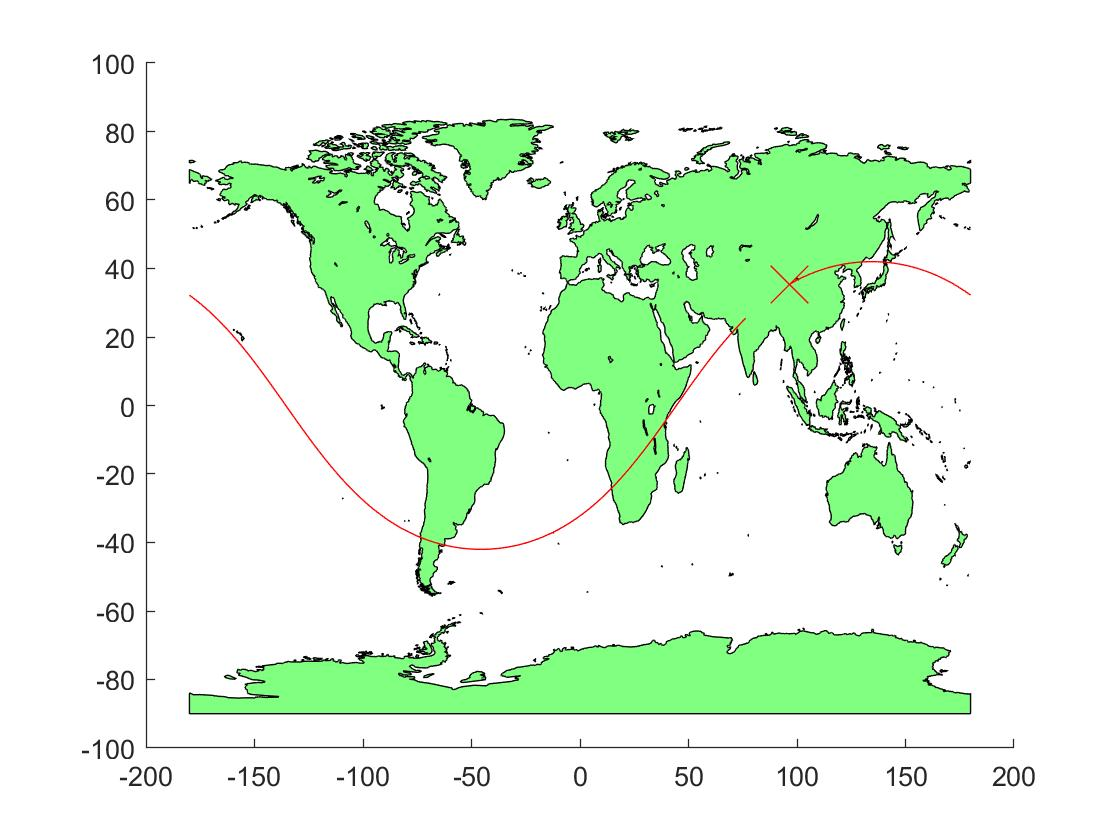
\includegraphics[scale=0.3]{MATLAB}
  \caption{MATLAB Geoshow Plot}
  \label{}
\end{figure}
Initial latitude and longitude:\\
$\phi = 35.4143^\circ, \lambda = 96.5763^\circ$\\
Final latitude and longitude:\\
$\phi = 25.4745^\circ, \lambda = 76.3665^\circ$\\
\vspace{5px}
\newpage
4. Use GMAT to produce a ground track of the orbit to confirm the MATLAB code.\\
\begin{figure}[!htb]
  \center
  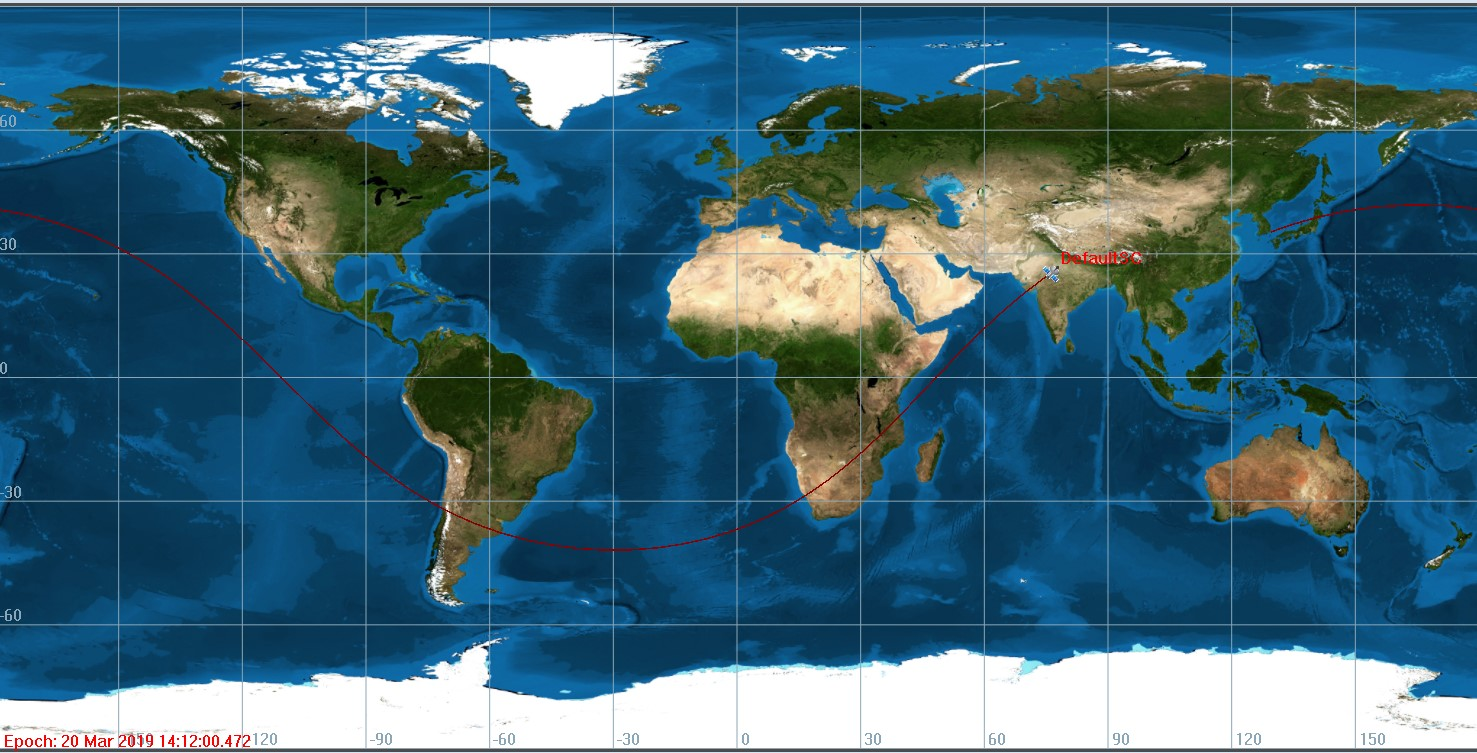
\includegraphics[scale=0.6]{GMAT}
  \caption{GMAT Spacecraft Plot}
  \label{}
\end{figure}
$\vec{r}_1^{ECI} = -2163.29 \hat{x} + 7099.49 \hat{y} + 3535.94 \hat{z}~km$\\
$\vec{v}_1^{ECI} = -4.72 \hat{x} - 4.52 \hat{y} + 3.05 \hat{z}~\frac{km}{s}$\\
\vspace{2px}
GMAT Initial latitude and longitude:\\
$\phi = 35.50^\circ, \lambda = 129.73^\circ$\\
GMAT Final latitude and longitude:\\
$\phi = 25.56^\circ, \lambda = 76.41^\circ$\\
The initial latitude is within $0.2^\circ$ but the initial longitude is not. This is unexpected becuase the GMAT final latitudes and longitudes are both within the $0.2^\circ$ limit.
This difference in initial longitudes is attributed to the fact that the matlab code did not take the rotation of the earth into account. This makes sense because the differe is only seen in the resulting longitude. To fix this error I would need to recalculate the Tu value at each new successive $\theta^*$
\vspace{5px}

\newpage
HW5.m
\begin{lstlisting}[frame=lines,style=Matlab-editor,basicstyle = \mlttfamily]
clc; clear all; close all

%constants
MU = 42828;

% Problem 1
vr = [-2089.6 -2515.7 -6382.0];
vv = [2.1744 0.76911 0.13452];

r = norm(vr)
v = norm(vv)

vh = cross(vr, vv);
h = norm(vh);

syms a
energy_eqn = v^2/2 - MU/r == -MU/(2*a)
energy = v^2/2 - MU/r
a = double(solve(energy_eqn, a))

syms e
h_eqn = h == sqrt(MU*a*(1-e^2))
e = double(solve(h_eqn,e))
e = max(e)

syms E
E_eqn = r == a*(1-e*cos(E));
E = double(solve(E_eqn,E));
E = -min(E) %Because it is descending.

syms time_since_p
time_since_p_eqn = sqrt(MU/a^3)*time_since_p == E - e*sin(E);
time_since_p = double(solve(time_since_p_eqn,time_since_p))

% Problem 2
p = h^2/MU;
true_a = -acos(p/(r*e) - 1/e)
vv_rt = [h*e/p*sin(true_a) h/r 0] % answer

% Problem 3
E1 = E;
t1 = time_since_p;
vr1 = vr;
vv1 = vv;
r1 = r;
v1 = v;
t2 = time_since_p + 12*60*60;
n = sqrt(MU/a^3);
M = n*t2;
E2 = fzero(@(x) x-e*sin(x)-M, 0);
f = 1 - a/r*(1-cos(E2-E1));
g = (t2 - t1) - sqrt(a^3/MU)*(E2 - E1 - sin(E2 - E1));

vr2 = f*vr + g*vv;
r2 = norm(vr2);
fdot = -sqrt(MU*a)/(r2*r1)*sin(E2-E1);
gdot = 1 - a/r2*(1-cos(E2-E1));

vv2 = fdot*vr1 + gdot*vv1 % intertial unit vectors

true_a2 = -acos(p/(r2*e) - 1/e)

vv2_rt = [h*e/p*sin(true_a2) h/r2 0] % radial-tangential

% Problem 4
vr2_peri = [r2*cos(true_a2) r2*sin(true_a2) 0]
vv2_peri = sqrt(MU/p)*[-sin(true_a2) e+cos(true_a2) 0]

% Problem 5

% find i theta omega
syms inc
h_hat = cross(vr2, vv2)/norm(cross(vr2, vv2))
inc_eqn = cos(inc) == dot(h_hat, [0 0 1])
inc = double(solve(inc_eqn,inc))
inc = max(inc)

syms RAAN
RAAN_eqn_1 = sin(RAAN)*sin(inc) == dot(h_hat, [1 0 0])
RAAN_eqn_2 = -cos(RAAN)*sin(inc) == dot(h_hat, [0 1 0])
RAAN1 = double(solve(RAAN_eqn_1));
RAAN2 = double(solve(RAAN_eqn_2));
RAAN = min(RAAN1)*180/pi

syms arg_peri
r1_hat = vr1/norm(vr1)
theta_hat = cross(r1_hat, h_hat)/norm(cross(r1_hat, h_hat))
syms theta
theta_eqn_1 = sin(inc) * sin(theta) == dot(r1_hat, [0 0 1])
theta_eqn_2 = sin(inc) * cos(theta) == dot(theta_hat, [0 0 1])
theta1 = double(solve(theta_eqn_1, theta))
theta2 = double(solve(theta_eqn_2, theta))
theta = intersect(theta1, theta2)
arg_peri_eqn = arg_peri == theta - true_a
arg_peri = double(solve(arg_peri_eqn, arg_peri))
\end{lstlisting}

\end{document}
